\documentclass[conference]{IEEEtran}

\usepackage{cite}
\usepackage{float}
\usepackage{multicol}
\usepackage{graphicx}
\usepackage{url}
\usepackage{hyperref}
\usepackage{epstopdf}
\usepackage{xcolor}
\usepackage{array}
\usepackage{booktabs}
\usepackage{xspace}
\usepackage{amsmath}
\usepackage{subfigure}

\setlength{\heavyrulewidth}{1.5pt}
\setlength{\abovetopsep}{4pt}

\newcommand{\ie}{\emph{i.e.,}\xspace}
\newcommand{\eg}{\emph{e.g.,}\xspace}

\begin{document}

\title{The Smart Grid and the Strategic Adversary: A Story of Peril and Promise}

\author{\IEEEauthorblockN{Nathan Burow, Saurabh Bagchi}
	\IEEEauthorblockA{School of Electrical and Computer Engineering \\ Purdue University \\ \{nburow, sbagchi\}@purdue.edu}
}

\maketitle

\begin{abstract}
One of the key benefits of the smart grid is the ability to integrate new power sources, most notably renewables.  However, these sources produces variable amounts of power, which makes fulfilling consumer demands challenging.  To offset this however, the smart grid will allow consumers to add flexibility to their demands.  This added flexibility will let the utility smooth demand and reduce peak demand by rescheduling flexible consumers to off peak times.  All of this will rely on the cyber component of the smart grid, which means that it is susceptible to malicious manipulation.  This paper examines a system with variable power supply and flexible consumer demand in the face of a limited, strategic adversary.  We model the game between the utility and the adversary and the utility to find the impact of various attacks, and who how much effect strategic defensive investments can have.  We find that the attacker can increase standby power usage by 50\%, and that our defensive strategy can halve this to 25\%.

\end{abstract}

\section{Introduction}
\label{Introduction}

It is trite but true that the power grid underlies most of modern civilization.  Traditionally the power grid has had a 
few fixed producers that sell power to utilities, who in turn distribute it to their customers.  Traditionally these 
customers have not coordinated with the utility, but simply bought whatever power they needed at the prevailing price.  
Similarily, utilities have simply ensured that they have enough power to meet their customer's demands.  
With the advent of the smart grid, this picture is giving way to dynamic supply and dynamic demand, incentivized in part by dynamic changes in price of energy.  Renewables like wind and solar will enter the supply side of the equation in greater numbers and will contribute to the variation in available supply, in a somewhat unpredictable manner. Increased connectivity through the smart grid will allow consumers (and more specifically, the smart appliances) to be 
aware of the prevailing price of energy and calibrate its usage accordingly. 

In the smart grid, consumers can also communicate their power demands and constraints to the utility, who can then schedule
power dispatch to them accordingly.  For example, if the communicated demand over the next time window (15 minutes out, one hour out, etc.) exceeds the anticipated supply, the utility may decide to fire up an expensive generator using fossil fuel. One crucial observation enabling this kind of dynamic demand-supply negotiation is that some demand loads are flexible (``elastic'' in economic-speak) in that they can be scheduled to run at any time within a time window. For example, running the dishwasher or charging an electric vehicle is flexible as long as it is completed by a certain time. Other kinds of loads, such as running the AC in the summer, are not flexible. In aggregate though, the presence of elastic loads will enable consumers to indicate flexible usage periods to the utility, and the utility to schedule its various sources of electricity in a price-optimal manner. This beneficial aspect of the smart grid has been expressed in many publications and even mainstream books (such as, Thomas Friedman's ``Hot, Flat, and Crowded'' from 2009). The scheduling problem for the utility has been investigated in many publications, many of which provide a theoretically rigorous treatment of the problem \cite{petersen2013taxonomy}. 

However, no prior work has investigated the impact of security attacks on such scheduling. Security attacks in the smart grid are widely anticipated \cite{nist} and many demonstrations have been done in laboratory settings \cite{hussain2012ncs}. It is till now unknown how security attacks --- jamming, false data injection, and delays in the communication channel --- affect the scheduling problem. The ultimate possible impact could be in the form of brownouts or blackouts and in our evaluation, we bring this out in the form of instantaneous mismatches between the demand the supply. A mismatch is undesriable in both directions --- if the demand is larger, this may lead to brownouts or blackouts, and if the supply is larger, then this may mean that the utility had to use more expensive sources of energy to fill a perceived (but ultimately incorrect) demand. The attacks could result in these impacts by disrupting the communication of the actual demand. Due to the interconnected nature of the smart grid, there are many possible entry points for such attacks --- the smart meters, the connection of these to the neighborhood data collection unit (DCU), the connection between the DCU and the control station at the local sub-station, etc. In addition to demonstrating the effect of such attacks, we take well-known security controls and evaluate how using them in our smart grid setting will mitigate the effects of some of these attacks. For example, we show that transient denial of service can be sucessfully ``fought through'' by using historical data of demand, even when the demand is somewhat fluctuating from day-to-day, provided a good characterization of the elasticity of the loads can be done. 

We build a discrete event simulator with two actors --- a strategic adversary and a defender (can be taken to model a utility). The adversary has a budget for the attack, in terms of the number of assets she can simultaneously target, and performs a game-theoretic determination of which assets to target subject to the budget constraint. The defender also performs a game-theoretic determination of which assets to make more secure against the above types of attacks. The discrete event simulation can model various intensities of attacks, different characteristics of loads, and different budgets for the adversary and the defender. For each configuration, it can provide the mismatch metric without any attack, with the attack and without any defense, and with the attack and with the defense controls in place. 

We find that two new classes of attack - changing the time constraints of customer demand, and adding constraints to customer demand - can have a signficant impact, increasing the mismatch by up to 50\%.  These two attacks directly target the amount of flexibility available to the utility when dispatching power to the consumer, and so serve to hgihlight the critical importance of that flexiblity to the system.  We propose defensive investments, like the addition of stronger cryptography (public key authentication) or physical measures (particuarly at substations) to prevent these attacks.  Our defensive strategy can halve the additional mismatch from the attack, which shows that systems designed with these new attack surfaces in mind can be robust to these new attack surfaces.  

We have released our simulator as an open source project, along with our simulation datasets at \cite{gridsec}.  The rest of the paper is organized as follows: Section \ref{Related Work} surveys existing work in the field, Section \ref{Model} details our model of the customers, power producers, utility, and adversary, Section \ref{Game} defines the strategic game between the adversary and the utility, Section \ref{Simulation} provides and overview of our simulator, Section \ref{Experimental Results} gives the details of our results, and Section \ref{Conclusion} concludes.

% SB (5/8/15): Point to some real deployment like this and some real instance of attack. 
% Nobody has shown how damaging an attack can be in such environments. We show that and show how relatively simple defense mechanisms based on prior work can mitigate these attacks. 
% Explain what destabilization means. 
% What are our defense strategies (in brief)?
% We provide a technique to evaluate how much damage can be caused under various different conditions - capabilities of the attacker, distribution of the load types
% Our simulation is a discrete event simulator which we open source.
% Key takeaways

\section{Model}
\label{Model}

We examine the smart grid over the course of a given day, divided into finite time steps (of an arbitrary granularity, the exact value of which does not affect our solution, except for the running time, which we are not considering here). Our model has three components: Power Generation, Consumers, and the Utility. Each of these components is characterized by their behaviors, goals, and constraints. Additionally, we present our model for how the power generators and the consumers communicate with the utility. 

\subsection{Power Generation}
\label{Power Generation}

We primarily consider power generated by renewable sources, such as wind and solar. These sources have a high degree of individual variation. However, we assume that there are sufficient sources from a wide enough geographic area that in aggregate they produce a normally distributed amount of power and that the mean of this supply distribution is the same as the mean of the demand distribution. This implies that under normal circumstances (no attack), in the average case, there will be neither any shortfall nor excess power. We also include a fossil fuel source that is capable of making up any short fall in production for a given time period and can be spun up fast. However, such a source is expensive, and therefore, its use should be minimized, as well as ecologically not very desirable. 

\subsection{Consumer}
\label{Consumer}

We model three different types of consumers, classified based on the flexibility of their demand. These classes are the same as in \cite{petersen2013taxonomy}. These consumers are primarily categorized based on the flexibility of their power demand. 
The first and most flexible class is buckets. Buckets are conceptually a heat sink and 
a simplified analogy is a house with a heat pump, which is used for energy storage and thus, energy can be tapped from the bucket. They are modelled as starting empty, and have a maximum rate at which it can be charged (a max power value) as well as a maximum rate at which it can be drained. As such, they can provide a reserve against production shortfalls, or a place to store excess production for the future. Each bucket has a maximum capacity, which determines how long it will take to be charged in an uninterrupted mode. 

The second class is batteries. A good example of this class is an electric vehicle that has been plugged in to charge overnight. As long as it has received a full charge by morning, one does not care when it charges. Further, it does not have to be charged continuously. A battery can only receive power from the grid, and (counter to what the common meaning is) cannot store and provide energy. It is contrained by the total amount of energy required, a maximum rate of charging, and a time by which that total energy is required.

The final, and least flexible class, is bakeries. Taking the obvious example: a bakery must produce bread by a certain time. Bread must be baked for a certain amount of time, and furthermore must be baked continuously. This means that like batteries bakeries face time and total energy constraints, but they add an additional constraint in that once they are started they must receive power every time step until they have completed their job.

\subsection{Communication}
\label{Communication}

The power generators communicate the amount of power they are currently producing to the utility at each time step. However, they have no forward knowledge of how much power they will produce at the next time step, and consequently neither does the utility. This is a pessimistic way of modeling the supply projection since in reality there will be some prediction of impending supply characteristics, say based on historic weather patterns. The consumer communicates each of its constraints when the load is created. This means the power, energy, and time constraints. We simplify this by assuming that all jobs are created at the beginning of the day. Customers can modify their job demands midstream, though in our model, this flexibility is only exploited by adversaries.

\subsection{Utility}
\label{Utility}

The utility has two inputs: the amount of power generated by the renewable sources, and the demands from the consumers, which are communiated to it as described above. The utility is required to meet all consumer demands. However, it is free to reschedule them to the greatest extent possible. Using this flexibility the utility's goal is simple: to ensure that all power generated is used, and to minimize the amount of power it has to receive from the fossil fuel backup. To do this, the utility uses the Agile Balancing scheduling algorithm in \cite{petersen2013taxonomy}. This algorithm computes an agility factor for each customer which reflects the number of ways remaining it can be scheduled.  It then provides power to any customer it is forced to (to meet the customer's constraints), and finally dispatches any remaining power to the customers in decreasing order of agility.  It uses the buckets as a sink for any excess production, or a source to make up any short fall, when possible.

\section{Two-Player Sequential Game: Utility and Adversary}
\label{Game}

\subsection{Game strategy}

We model our system as a single stage concurrent game, where the adversary and then the utility simultaneously make their moves. The adversary seeks to maximally disrupt the grid by making strategic use of a budget for the total number of assets that she can target. The utillity estimates the high-valued targets and probabilistically makes a restricted set of all of its assets more resilient. We assume that the adversary model is estimated by the utility in so far that it knows that the adversary has a preference for targeting high-valued assets, though the adversary's and the utility's choices are both probabilistic and thus, there is unlikely to be an exact match of the assets. In our context, the adversary seeks to disrupt the communication between a load point and the utility, so that the utility has less information for its scheduling decision. The value of an asset for the purpose of attack or defense is given by its flexibility (bucket > battery > bakery), the energy and power demand (higher means higher value), and the time constraint (less constrained means higher value).  
There are three experimental settings that we explore - a baseline where there is no adversary, a game where only the adversary makes a move, and a game where both the adversary and the utility (simultaneously) make a move. We characterize how much the mismatch is in settings 2 and 3 relative to the baseline and observe how much setting 3 is improved over setting 2. 

If all the assets are ordered from low to high flexibility and there are a total of $n$ assets, then the probability of attacking, or defending, asset $i$ is given by Equation \ref{probability}. This gives a gradually increasing probability of attacking assets that have higher flexibility. 

\begin{equation}
\label{probability}
Pr(\text{Attack asset } i) = \frac{i}{\sum\limits_{j=1}^n j}
\end{equation}


\begin{table}[!htbp]
\label{strategies}
\centering
\begin{tabular}{p{2cm} | p{3cm} | p{3cm}}
\toprule
Class & Adversary & Utility\\
\midrule
Jamming & Attacker jams a subset of the bakeries and disrupts communication of the demand to the utility. ({\bf Jam}) & Utility uses historical data and daily fluctuation for any given bakery is $\pm$20\%  ({\bf Jam-Defense})\\
False Data Injection - Load &  Attacker increases the load of a subset of bakeries by 20\% ({\bf FDI - Load}) & Utility encrypts communications with a subset of bakeries, preventing them from being attacked ({\bf FDI - Load Defense}) \\
False Data Injection - Time & Attacker changes the timing constraint of a subset of bakeries such that they all must run at the same time ({\bf FDI - Time}) & Utility encrypts communications with a subset of bakeries, preventing them from being attacked ({\bf FDI - Time Defense})\\
False Data Injection - Class & Attacker permutes a subset of buckets into bakeries ({\bf FDI - Class}) & Utility encrypts communications with a subset of the buckets such that they cannot be permuted ({\bf FDI - Class Defense})\\
\bottomrule
\end{tabular}
\caption{Attack and Defense Strategies}
\end{table}

\subsection{Operational Rules}
\label{Rules}

At the beginning of the day, the customer's send their demands to the utility. These are visible to the adversary, but he cannot modify them in transit (\ie they are protected by HMAC or similar), other than by jamming the customer and causing the packet to be lost in transit.   Once the customer messages are received, the adversary can inject any modification messages that he wants, subject to the model in \ref{Adversary}. At that point the day begins, and the power producers send their production to the utility, who distributes it according to \ref{Utility}. The power plant and utility continue in this fashion for every time step until the end of the day. At the end of the simulation period, the total cost that the adversary inflicted
on the utility is determined, as measured by adding up the mismatch between the actual demand and the supply for each time step. 

\subsection{Adversary}
\label{Adversary}

The adversary's goal is to force the utility to either waste power in case of lower demand than supply, or have to use power from the fossil fuel run backup. To do this we present an adversary model in Table \ref{strategies}, based on jamming or false data injection. The idea of jamming \cite{gupta2010optimal}, and false data injection on loads \cite{lin2012false}\cite{yuan2011modeling} are well-established in the energy grid literature, though it is novel in this context of heterogeneous loads. The false data injection on time constraints and consumer classification are new extensions on false data injection made possible by the presence of heterogenous customers.

\begin{itemize}
\item {\em Jamming}. The attacker can jam communication between the utility and producers or consumers (we only use consumers for this, and the subsequent attacks). We model this in terms of the number of customers prevented from communicating with the utility, divorced from any specific topology. We assume that the attacker can jam a percentage of the utility's customers. This is not a stealthy attack: the utility can tell that the communication channel has been jammed.

\item {\em False Data Injection - Load}. The attacker can modify the communicated demand from consumers or supply from producers. Here the attacker can remain stealthy by carefully crafting the attack, such as, the amount of change introduced \cite{yuan2011modeling}. It is shown that under these conditions, there is no statistical method for detecting this attack. For our purposes, we assume that the attacker can increase the demand by 20\%. 

\item {\em False Data Injection - Modify Time Constraints}. Here the attacker can change the consumer's time constraints, \ie he can cluster the demands more tightly. This can signfiicantly decrease the flexibility available to the utility by forcing power to be distributed to many customers at the same time. We assume a straightforward extension of \cite{yuan2011modeling} such that there is no known statistical method for detecting this attack.  We assume an aggressive attacker that removes as much of the flexibility in the time to completion as possible.

\item {\em False Data Injection - Change Customer Class}. Buckets are very useful to the utility in scheduling because they provide
the most additional flexibility. The attacker targets them by adding constraints such that the buckets become bakeries, \ie has to run continuously, has a definite finish time, and utility cannot draw energy from it.  Here we allow the attacker to modify a percentage of the buckets, as detailed in \ref{Simulation}.  We assume sufficient variety in the composition of the customers that this modification cannot be detected with any known technique, if the adversary targets a small enough percentage of buckets for this class change. 

\end{itemize}

\subsection{Utility}
\label{Utility2}

The utility's core strategy is to detect and correct for any malicious communications. This will allow its performance to be
constrained solely by its scheduling algorithm (our baseline) and not by the attacker. However, only the jamming attack is detectable by the utility, assuming the attacker follows the constrainst set forth in \cite{yuan2011modeling}. Consequently, the best that the utility can do against the other attacks is to make defensive investments. The utility knows the attacker's strategy and picks a subset of the assets to defend, ordering it in priority as the adversary does, \ie a load with higher flexibility gets higher priority. The exact budget of the utility, in terms of the number of assets it can defend, is a simulator parameter and can be less than, equal to, or greater than that of the adversary. The utility's defense is to employ stronger (and therefor more expensive) cryptography when communicating with the defended customer.  An example would be adding public key authentication. This defense is assumed to be too burdensome for general deployment, but practical enough for limited use as a defense. The burden comes primarily from having to distribute keys, refresh them periodically, and remove keys in case of some compromised end points.  

\begin{itemize}
\item Jamming. Jamming is always detected. The utility corrects for this by using historical data. The historical load data is accurate to within 20\%.  
% This means that the jamming attack may actually ease the scheduling problem (by decreasing load), though even in this case it would lead to brownouts as customers receive less power than they require (this effect is left for future work).  
Note that we assume that the constraints in the historical data are accurate. That is, if if a customer was a battery before being jammed, a customer is a battery afterwards, and has the same time constraint.

\item False Data Injection - All Varieties. The utility cannot actively defend itself against this attack, because there is no known technique to detect it assuming the adversary stays within its limits. The utility can, however, model the adversary's likely targets and defend them against attack, as described above, by strengthening some assets. This passive defense further limits the amount of damage that the attacker can inflict. If the utility were to institute a policy that all constraints (load, time, constant power) could only be relaxed (decreased, delayed, removed) at specific periodicities, then these attacks would become less damaging. However, we consider such policies to be too constraining on customers, and unlikely to be deployed.

\end{itemize}

\section{Simulator Implementation}
\label{Simulation}

This section provides a brief overview of our open source simulator \cite{gridsec}, describing its parameters and use.  The simulator takes as command line arguments how long the simulation is, a seed for its random number generator, which attack model to use, and what percent of the customers the attacker can effect.  It outputs the amount of power either wasted (positive number) or required from backup sources (negative number).  It gives three such results: the baseline result without the attack, the result with the attack, and the result with both the attack and defense.

Internally, the renewable energy producers are modeled collectively.  We assume that there are sufficiently many of them that the central limit theorem applies and they are normally distributed in aggregate.  Consequently, we sample from a normal distribution at each time step to find the amount of power produced.  The mean and median of this distribution are tunable in the code, and are members of the Simulator class.

The number of Bakeries, Batteries, and Buckets is tunable in the code, with members of the Simulator class for each.  When initializing them, we first calculate the total amount of power available, on average, over the simulation by multiplying the mean of the producers by the simulation run time.  This is then divided by the total number of customers to get the mean power required per customer.  We again assume that the customers in aggregate follow a normal distribution as per the central limit theorem.  The standard deviation of this distribution, expressed as a percentage of the mean, is a user tunable member of the Simulator class.  We sample this distribution once for each customer to get the amount of power actually required for the customer.  Note that this implies that on average the amount of power demanded and supplied is equal, which makes the scheduling problem tractable.  We then calculate the minimum amount of energy each customer must receive per time step to statisfy his total demand. We increase this amount of energy by a random percentage, and based on this energy per time step compute the earliest time that the customer could be finished.   We then select the actual required finish time (for Bakeries and Batteries) uniformly over [earliest, simulation end].  

As mentioned abover, the percent of customers that can be attacked is a parameter to the simulator.  This is used to calculated the actual number of customers attacked.  We make the simplifying assumption that the number of customers attacked is less than the number of Bakeries for the Jam, False Data Injection - Load, and False Data Injection - Time attacks.  This allows our adversary model to only consider Bakeries for those attacks.  Bakeries are the most constrained customers, so attacks against them are the most damaging.  For the False Data Injection - Class attack we assume that there are sufficient Buckets in the system so that only Buckets are attacked.  As above, turning a Bucket into a Bakery (most flexible into least flexible) is the most damaging attack.

% SB (5/10/15): Say something about the characteristics of each kind of load - their power, energy, and time constraints.

\section{Experimental Results}
\label{Experimental Results}

We used the simulator to examine the results of the game between the adversary and the utility described in Section \ref{Game}. We examined the effectiveness of the four adverserial strategies and the corresponding defense mechanisms presented earlier (Table \ref{strategies}). In the first scenario, there are an equal number of each class of customer. In the second, 40\% are Bakeries, 40\% are Batteries, and the remaining 20\% are Buckets. In both scenarios, we assume that the attacker and the utility have the same budget, \ie they can attack or defend the same number of customers. All of our results are over 15,000 total customers. The results presented here are averaged over 10 different random number seeds in order to eliminate any bias in a given sample from the distributions. 
The metric that we are interested in is the mismatch between the supply and the demand at the utility, summed up over all the time steps of the simulation (we had 100 time steps for these results). A greater mismatch means worse impact of the attack. We provide the result as percentage change from the baseline, which is the case with no attack. So a greater change means a worse result. 

\begin{figure*}[htp]
    \centering
    \subfigure[Scenario 1: Equal proportion of load types - Bakeries, Batteries, and Buckets]{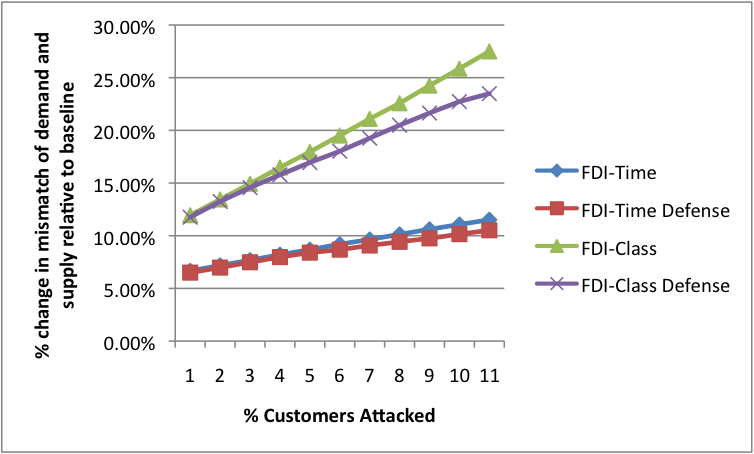
\includegraphics[width=.5\textwidth]{naieve-equal-attacks.png}}\hfill
    \subfigure[Scenario 2: 40\% Bakeries, 40\% Batteries, 20\% Buckets]{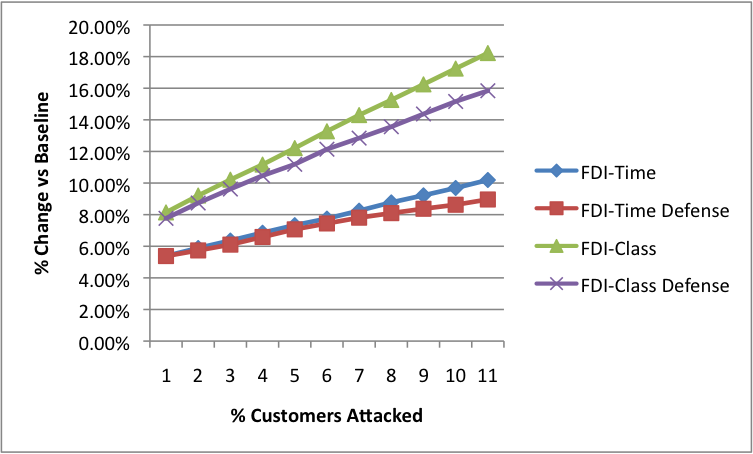
\includegraphics[width=.5\textwidth]{naieve-unequal-attacks.png}}  
    \caption{Results for the Na\"\i ve Adversary. A mismatch between supply and demand is undesirable for the utility. The greater the mismatch is relative to the baseline (no attack) (the Y-axis), the worse is the impact of the attack.}
    \label{naive}  
\end{figure*}

We first considered a na\"\i ve adversary who picks from among all the customers in a uniform random manner. To even the scales, we also had the utility choose assets to defend in a uniform random manner. In this case neither the Jamming nor the FDI-Load attack had any significant effect, and so are omitted from Figure \ref{naive}. Our defense is relatively ineffective against the na\"\i ve attacker, because of the random choices made by the adversary. However, the attack itself is also far less effective: only increasing the mismatch by 28\% in the worst case versus 52\% for the strategic adversary. The FDI-Class attack is more effective than the FDI-Time attack underlining how important the flexibility of buckets is to the utility for its load scheduling. 

Given this na\"\i ve baseline, we examined how much more effective a \emph{strategic} adversary is. In particular, the adversary preferentially targets the loads that have higher flexibility. In our simulation setting, this leads to the situation that only bakeries are targeted for all attacks other than the FDI-Class where it converts some buckets into bakeries. Figure \ref{strategic} show.

\begin{figure*}[htp]
    \centering
    \subfigure[Scenario 1: Equal proportion of load types - Bakeries, Batteries, and Buckets]{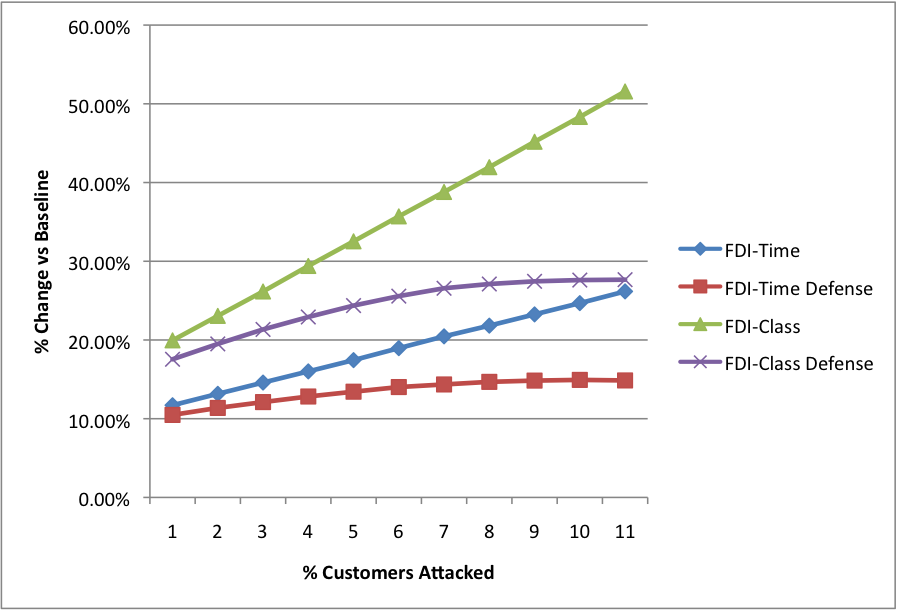
\includegraphics[width=.5\textwidth]{equal-attacks.png}}\hfill
    \subfigure[Scenario 2: 40\% Bakeries, 40\% Batteries, 20\% Buckets]{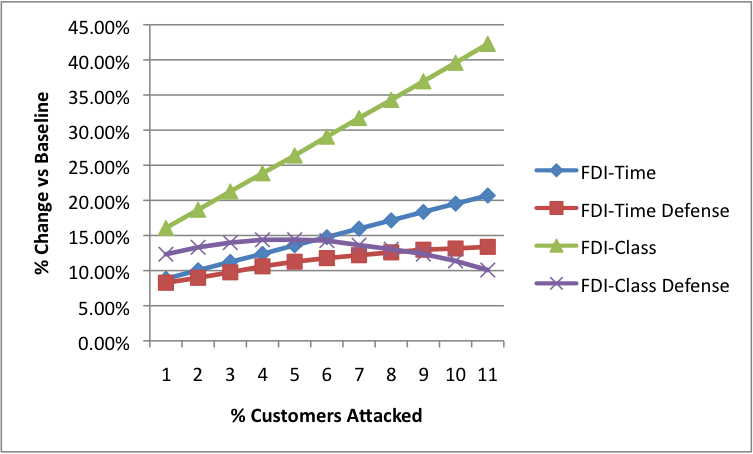
\includegraphics[width=.5\textwidth]{unequal-attacks.png}}  
    \caption{Results for the Strategic Adversary. A mismatch between supply and demand is undesirable for the utility. The greater the mismatch is relative to the baseline (no attack) (the Y-axis), the worse is the impact of the attack.}

    \label{strategic}  
\end{figure*}

Again, the FDI-Load and Jam attacks are not effective, and are omitted from our results. This means that the low level of FDI-Load to remain stealthy makes it such that existing scheduling is not perturbed by it. However, the strategic attacks, FDI-Class and FDI-Time, have a significant impact, increasing mismatch by 52\% in the worst case. However, our defense was able to blunt the strategic adversary back down to the efficacy of the na\"\i ve, random adversary. This is a significant decrease: dropping the attacker induced mismatch from 52\% to 28\% of baseline. 
The other notable result is that the efficacy of our defense against the FDI-Class attack \emph{increases} as more customers are attacked. This attack targets Buckets, the most flexible type of customer, and turns them into Bakeries, the least. The efficacy of our defense, which preserves Buckets, underscores the critical nature of the flexibility they provide to the utility. 



\section{Related Work}
\label{Related Work}

We build on the model for flexible consumer demand presented by Petersen et al \cite{petersen2013taxonomy}. There are three classes of consumers: Buckets, Batteries, and Bakeries. Buckets can both accept power from the grid, or push power back into the grid, and so are the most flexible class of consumer. Batteries must be charged to a certain level by a given time, but do not need power constantly while charging (think of an Electric Vehicle: it needs to be charged by the next morning but it does not need to charge constantly). Bakeries are the most constrained class of customer: adding a requirement for constant charging to the Battery constraints.

Other prior works have looked at attacks made possible by the introduction of the smart grid, but they do not consider consumer diversity. Chen et al \cite{chen2015detection} present a scheme for detecting false data injection attacks through deviations in spatial / temporal relationships of data. Lin et al \cite{lin2012false} examine the effects of false data injection on routing power in the smart grid. Yuan et al \cite{yuan2011modeling} examine similar attacks against the smart grid, and provide a set of equations that show how much and where an attacker can alter the load in the system while still remaining undetected. Sridhar et al \cite{sridhar2014model} present a model-based attack detection scheme that focuses on modulating the frequency of the grid in the face of false data injections. Teixeira et al \cite{teixeira2014security} provide a game theoretic model of a stealthy attacker who can alter line voltage readings, and present strategies for altering the configuration of substations to limit the set of stealthy attacks. 

Other classes of attacks have been examined in the literature, agian without considering consumer diversity. The DETER testbed has been used to examine the effects of DDoS attacks against smart grids \cite{hussain2012ncs}. Gupta et al \cite{gupta2010optimal} presented a limited, strategic adversary who could jam a certain number of communications channels, and presented optimal strategies for such an adversasry. 

Prior work has also considered how best to model risks introduced by the cyber component of smart grids. Ten et al \cite{ten2010cybersecurity} present a survey of existing work on the security of smart grids at the time, and present a risk assessment framework. Kundur et al \cite{kundur2010towards} show a methodology for modeling the grid and its interdependencies as a graph, which allows automated impact analysis. In our prior work, we presented a tool for risk assessment of advanced metering infastructure \cite{shawly2014risk}.


\section{Conclusion}
\label{Conclusion}

The smart grid provides greater flexiblity to the utility by recognizing inherent difference between customer's power demands, and this flexibility in turn helps the utility integrate new sources of energy, like renewables, that provide a fluctuating supply of power.  The problem for the utility is to schedule customers' demands and make the best possible use of renewable power (by minimizing both the amount of standby power used, and the amount of generated power that is not dispatched).  The additonal communication from customers to the utility - about their demand and its constraints - provides a new attack surface to malicious adversaries.  We find that in the worst case even a strategically limited adversary can increase the amount of standby power requried by 50\%.  Our proposed defensive strategy for the utility - to model what the adversary will likely attack and protect those assets - can cut this worst case number by at least half.

{\footnotesize
\bibliographystyle{IEEEtran}
\bibliography{references}
}

\end{document}
